\subsection{Miller effect}

Considering a basic feedback amplifier (such as the ones on the photoreceptors looked at previously), the parasitic drain capacitance $C_m$ is amplified by the gain of the amplifier (see figure \ref{fig:MillerEffect}). Therefore for the input node to charge the gate $V_1$ to a particular voltage it has to supply that much more charge, which limits how much you can speedup its response by increasing the gain.

\begin{figure}[H]
    \centering
    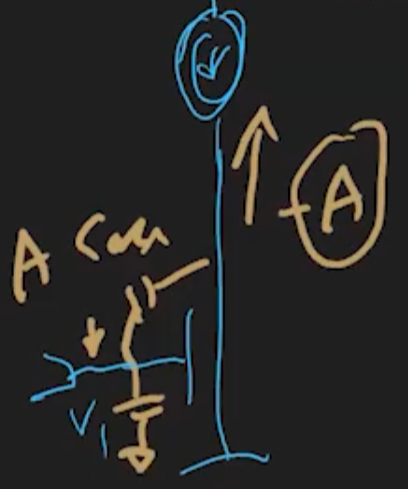
\includegraphics[width=0.6\linewidth]{../../Figures/miller_effect.png}
    \caption{The miller effect on feedback amplifier. Beautifully drawn by Tobi.}
    \label{fig:MillerEffect}
\end{figure}

By adding a second transistor right above the first one, we can circumvent the Miller effect (see figure \ref{fig:Cascode}).

\begin{figure}[H]
    \centering
    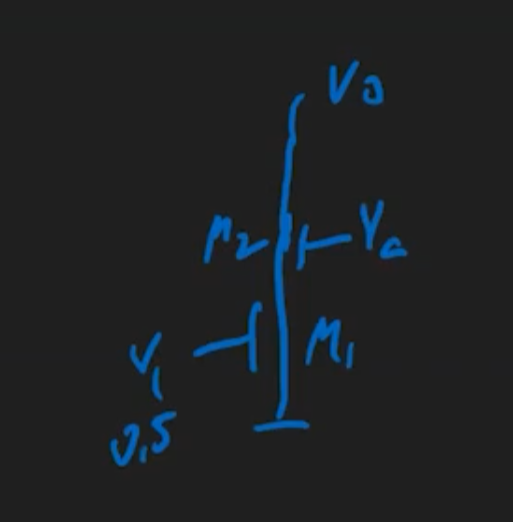
\includegraphics[width=0.6\linewidth]{../../Figures/cascode.png}
    \caption{Cascode to shield the amplifier from the miller effect. Beautifully drawn by Tobi.}
    \label{fig:Cascode}
\end{figure}
 